\newproblem{08a}
{
      Graph the line with slope $\dfrac{-2}{3}$ that passes through the point $(-4, 1)$. Label your axes and put number values on them. Identify at least three points on your line.\begin{onlyproblem}\begin{center}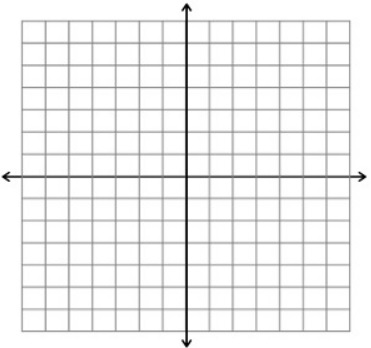
\includegraphics{fig-graphpaper.png}\end{center}\end{onlyproblem} \begin{onlysolution}\begin{center}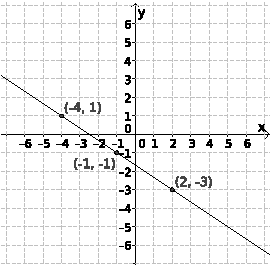
\includegraphics{fig095-08-a-answer}\end{center}\end{onlysolution}
}
{
	\begin{tabular}{l r}
	1 point for correct labeling of axes and number on them.\\
	3 points for correctly identifying 3 pts.\\
	1 points for the correct line.\\
	\end{tabular}
}

\newproblem{08b}
{
	Graph the line with slope $\dfrac{-2}{3}$ that passes through the point $(2, -1)$. Label your axes and put number values on them. Identify at least three points on your line.\begin{onlyproblem}\begin{center}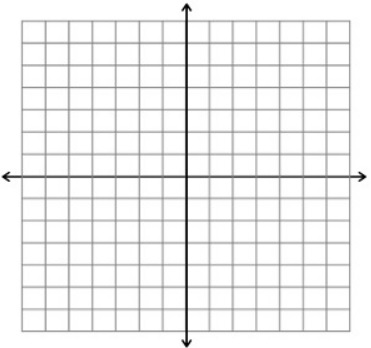
\includegraphics{fig-graphpaper.png}\end{center}\end{onlyproblem} \begin{onlysolution}\begin{center}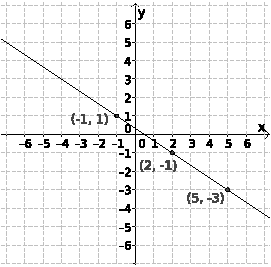
\includegraphics{fig095-08-b-answer}\end{center}\end{onlysolution}
}
{
	\begin{tabular}{l r}
	1 point for correct labeling of axes and numbers on them.\\
	3 points for correctly identifying 3 pts.\\
	1 pt for the correct line.\\
	\end{tabular}
}

\newproblem{08c}
{
	Graph the line with a slope $\dfrac{-3}{4}$ that passes through the point $(-1, 2)$. Label your axes and put number values on them. Identify at least three points on your line.\begin{onlyproblem}\begin{center}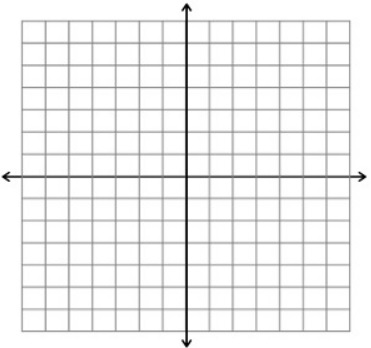
\includegraphics{fig-graphpaper.png}\end{center}\end{onlyproblem} \begin{onlysolution}\begin{center}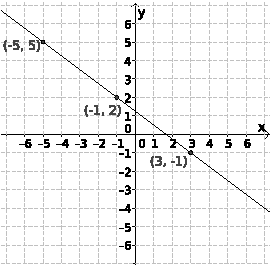
\includegraphics{fig095-08-c-answer}\end{center}\end{onlysolution}
}
{
	\begin{tabular}{l r}
	1 point for correct labeling of axes and numbers on them.\\
	3 points for correctly identifying 3 pts.\\
	1 pt for the correct line.\\
	\end{tabular}
}

\newproblem{08d}
{
	Graph the line with a slope $\dfrac{-2}{5}$ that passes through the point $(-1, 2)$. Label your axes and put number values on them. Identify at least three points on your line.\begin{onlyproblem}\begin{center}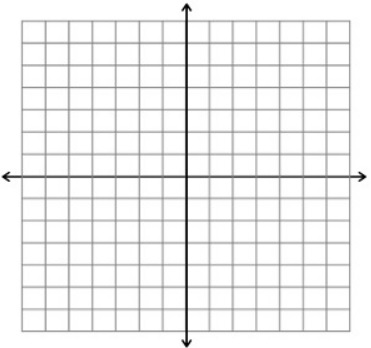
\includegraphics{fig-graphpaper.png}\end{center}\end{onlyproblem} \begin{onlysolution}\begin{center}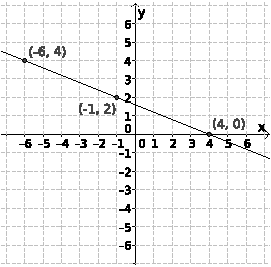
\includegraphics{fig095-08-d-answer}\end{center}\end{onlysolution}
}
{
	\begin{tabular}{l r}
	1 point for correct labeling of axes and numbers on them.\\
	3 points for correctly identifying 3 pts.\\
	1 pt for the correct line.\\
	\end{tabular}
}
